\chapter{PHÂN TÍCH QUY TRÌNH NGHIỆP VỤ BẰNG SƠ ĐỒ HOẠT ĐỘNG}

\section{Quy trình Đăng nhập và xác thực phân quyền người dùng (Activity Login)}

Quy trình xác thực người dùng bắt đầu khi người dùng gửi thông tin thông tin đăng nhập (username và password) đến API Backend. Hệ thống truy vấn CSDL để tìm người dùng tương ứng, kiểm tra trạng thái hoạt động (is\_active) và đối chiếu băm mật khẩu bằng Argon2. Nếu xác thực thành công, hệ thống sinh mã JSON Web Token (JWT) có đính kèm thông tin vai trò (role) gửi về cho Client lưu vào bộ nhớ an toàn.

Sơ đồ hoạt động chi tiết của quy trình đăng nhập được thể hiện tại Hình 4.1.

\begin{figure}[h!]
\centering
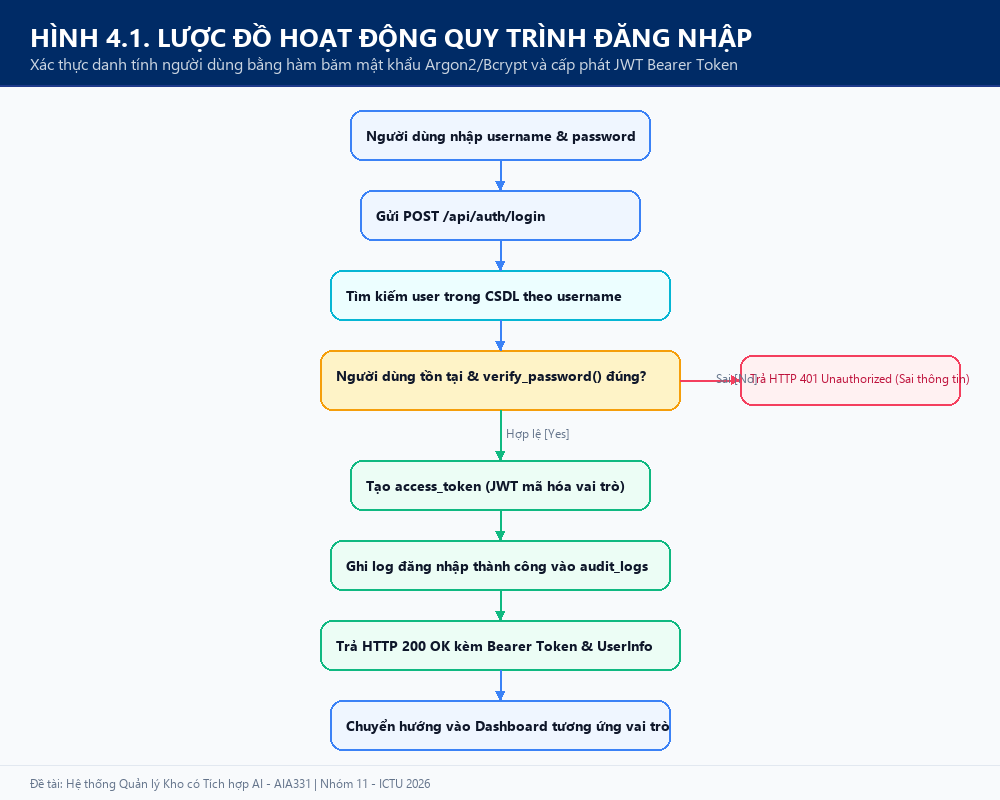
\includegraphics[width=0.92\textwidth]{figures/activity_login.png}
\caption{Sơ đồ hoạt động quy trình Đăng nhập và kiểm tra phân quyền RBAC}
\end{figure}

\section{Quy trình Lập và duyệt phiếu Nhập kho (Activity Import)}

Quy trình nhập kho bắt đầu khi thủ kho chọn nhà cung cấp và nhập danh sách các mặt hàng cùng số lượng, đơn giá nhập. Backend mở một giao dịch cơ sở dữ liệu (Database Transaction), tạo bản ghi phiếu nhập (import\_receipts), thêm các dòng chi tiết (import\_receipt\_details), đồng thời cập nhật tăng số lượng tồn trong bảng inventory và ghi bản ghi nhật ký biến động kho (stock\_movements). Toàn bộ thao tác được thực hiện theo nguyên tử (Atomic Commit).

Sơ đồ hoạt động quy trình nhập kho được minh họa tại Hình 4.2.

\begin{figure}[h!]
\centering
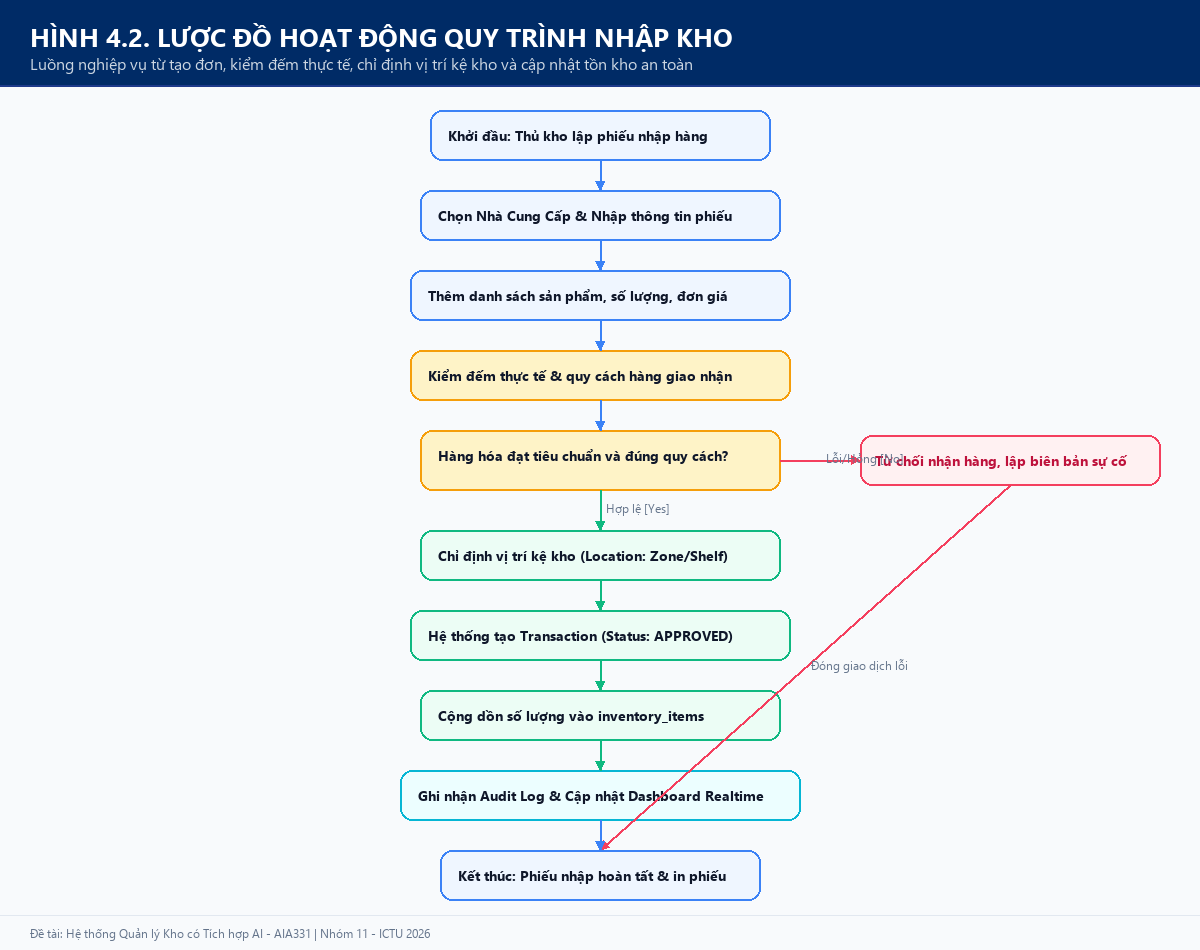
\includegraphics[width=0.92\textwidth]{figures/activity_import.png}
\caption{Sơ đồ hoạt động quy trình Nhập kho và cập nhật tăng tồn kho tự động}
\end{figure}

\section{Quy trình Lập phiếu Xuất kho và cơ chế kiểm soát âm kho (Activity Export)}

Quy trình xuất kho đòi hỏi tính kiểm soát an toàn nghiêm ngặt nhất trong hệ thống. Khi thủ kho gửi danh sách hàng cần xuất, Backend tiến hành kiểm tra tồn kho khả dụng hiện tại của từng mặt hàng:

- Nếu bất kỳ mặt hàng nào có số lượng xuất lớn hơn số lượng tồn hiện có, hệ thống ngay lập tức từ chối yêu cầu, hủy bỏ toàn bộ giao dịch (Rollback) và trả về thông báo lỗi HTTP 400 'Số lượng tồn kho không đủ để xuất'.

- Nếu tất cả mặt hàng đều thỏa mãn điều kiện tồn, hệ thống trừ số lượng tồn tương ứng, ghi nhận phiếu xuất (export\_receipts), lưu chi tiết xuất (export\_receipt\_details) và ghi nhật ký xuất kho vào stock\_movements.

Sơ đồ hoạt động quy trình xuất kho được thể hiện tại Hình 4.3.

\begin{figure}[h!]
\centering
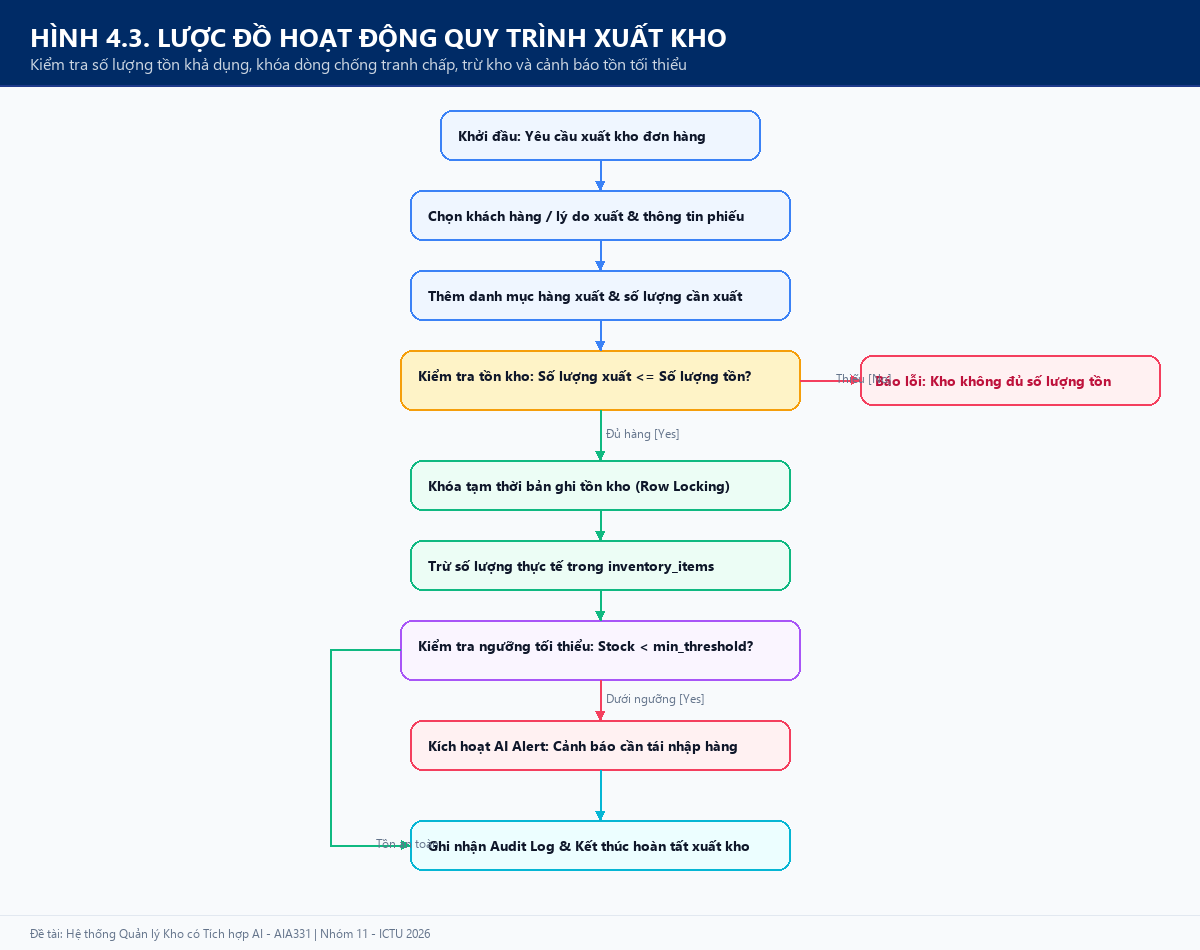
\includegraphics[width=0.92\textwidth]{figures/activity_export.png}
\caption{Sơ đồ hoạt động quy trình Xuất kho và cơ chế phòng chống âm kho}
\end{figure}

\section{Quy trình Phân tích số liệu và cảnh báo thông minh bằng AI (Activity AI Flow)}

Quy trình phân tích AI được kích hoạt tự động theo định kỳ hoặc theo yêu cầu của người quản lý. Hệ thống thực hiện truy vấn tổng hợp số liệu nhập xuất tồn trong 30 ngày gần nhất, tạo bản ghi JSON Snapshot. Bản ghi này được chuyển tới AIService để tính toán tốc độ tiêu thụ, dự báo số ngày hết hàng và phát hiện bất thường. Báo cáo định dạng Markdown sau đó được gửi về cho người dùng và hiển thị trên giao diện AI Analytics Hub.

Sơ đồ hoạt động quy trình phân tích AI được minh họa tại Hình 4.4.

\begin{figure}[h!]
\centering
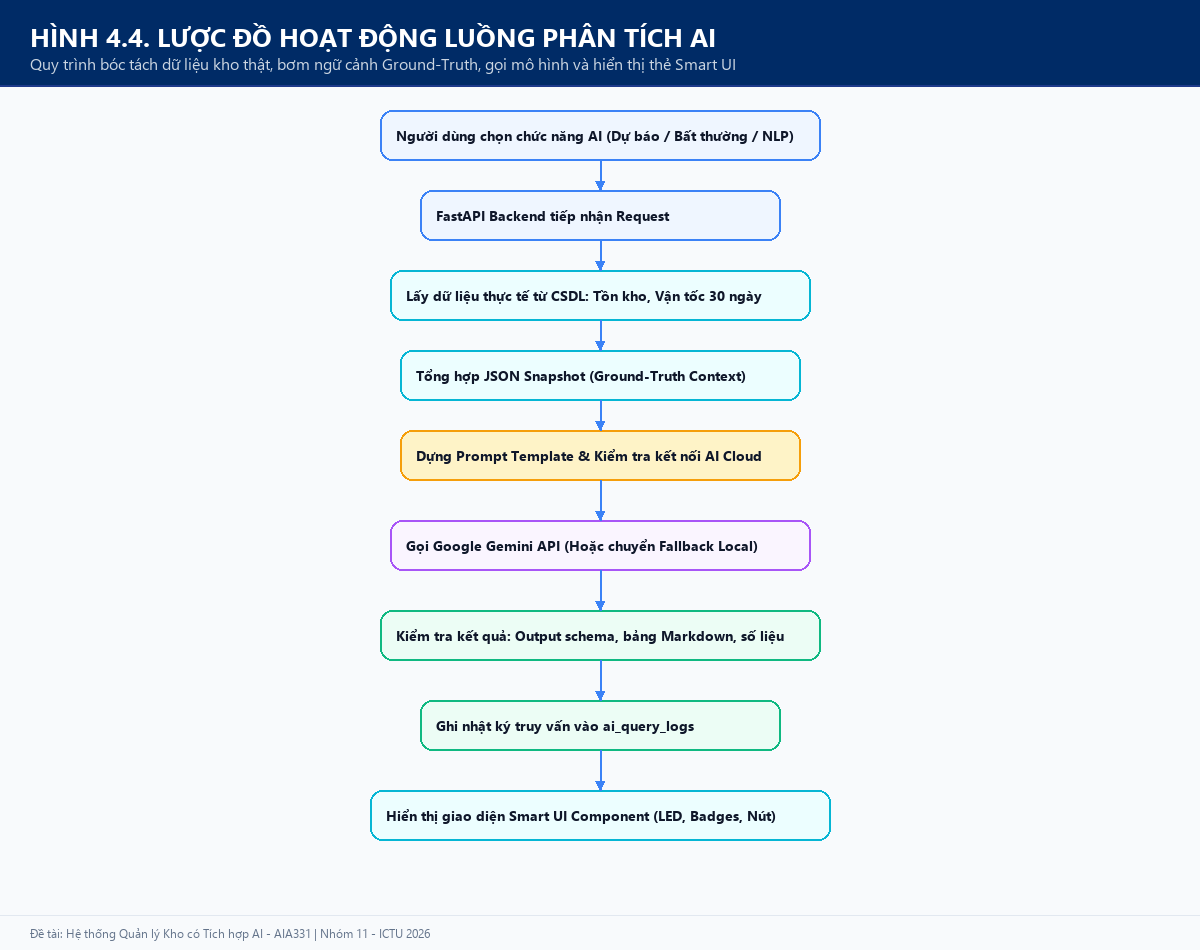
\includegraphics[width=0.92\textwidth]{figures/ai_flow.png}
\caption{Sơ đồ hoạt động quy trình Phân tích dữ liệu và sinh cảnh báo kho AI}
\end{figure}

